% =============================================================================
% AI/ML-Enhanced Crowdsourced Flood Validation System
% IEEE Conference Paper Template
% =============================================================================

\documentclass[conference]{IEEEtran}

% Packages
\usepackage{cite}
\usepackage{amsmath,amssymb,amsfonts}
\usepackage{algorithmic}
\usepackage{graphicx}
\usepackage{textcomp}
\usepackage{xcolor}
\usepackage{hyperref}
\usepackage{booktabs}
\usepackage{multirow}

% Custom commands
\newcommand{\todo}[1]{\textcolor{red}{[TODO: #1]}}

\begin{document}

\title{AI/ML-Enhanced Crowdsourced Flood Validation System Using DEM-Based Terrain Analysis}

\author{
\IEEEauthorblockN{Author 1\IEEEauthorrefmark{1}, Author 2\IEEEauthorrefmark{1}, Author 3\IEEEauthorrefmark{1}, Author 4\IEEEauthorrefmark{1}, Author 5\IEEEauthorrefmark{1}}
\IEEEauthorblockA{\IEEEauthorrefmark{1}Department of Computer Science and Engineering\\
University Name, City, India\\
Email: \{author1, author2, author3\}@university.edu}
}

\maketitle

% =============================================================================
\begin{abstract}
Crowdsourced flood reports from mobile applications provide real-time situational awareness during disasters but suffer from noise, false positives, and malicious submissions. We propose a novel three-layer validation algorithm that combines (1) physical plausibility checks using Digital Elevation Models (DEM) and Height Above Nearest Drainage (HAND), (2) statistical consistency analysis through spatio-temporal clustering, and (3) a Bayesian user reputation system. Evaluated on synthetic datasets simulating flood scenarios in the Mahanadi Delta, Odisha, our approach achieves 100\% precision and 100\% recall at 15\% noise level, with robust performance (98.5\% F1-score) even at 30\% noise. The system includes a FastAPI backend, React-based web dashboard for emergency coordinators, and demonstrates the effectiveness of multi-layer validation for disaster response.
\end{abstract}

\begin{IEEEkeywords}
flood validation, crowdsourcing, DEM, HAND, disaster management, machine learning
\end{IEEEkeywords}

% =============================================================================
\section{Introduction}
\label{sec:introduction}

Floods are among the most devastating natural disasters, affecting millions annually and causing substantial economic losses. In India, the Mahanadi Delta in Odisha is particularly vulnerable, experiencing recurring floods during cyclone season that cause significant loss of life and property. During these disasters, real-time situational awareness is critical for effective emergency response and resource allocation.

Crowdsourced flood reports from mobile applications offer a promising solution for ground-truth data collection, enabling citizens to report flooding conditions directly from affected areas. However, these systems face three fundamental challenges: (1) \textbf{noise} from inaccurate GPS and user error, (2) \textbf{false positives} from misidentification of normal water bodies as floods, and (3) \textbf{malicious reports} from deliberate misinformation. Without robust validation mechanisms, emergency coordinators cannot trust crowdsourced data for critical decision-making.

Existing validation approaches rely primarily on either statistical outlier detection or simple heuristics, failing to leverage the rich geospatial context available from Digital Elevation Models (DEM). We propose a novel three-layer validation algorithm that combines physical terrain analysis, statistical consensus mechanisms, and user reputation tracking to achieve robust flood report validation even in adversarial conditions.

\subsection{Problem Statement}
Crowdsourced flood reports offer real-time ground truth but introduce challenges:
\begin{itemize}
    \item \textbf{Noise}: Inaccurate GPS, user error
    \item \textbf{False Positives}: Misidentification of flooding
    \item \textbf{Malicious Reports}: Deliberate misinformation
\end{itemize}

\subsection{Contributions}
Our key contributions are:
\begin{enumerate}
    \item A three-layer validation algorithm combining physical, statistical, and reputation-based checks
    \item Integration of 30m FABDEM and HAND analysis for terrain-aware validation
    \item An offline-capable Progressive Web App for field deployment
    \item Comprehensive evaluation on synthetic datasets with varying noise levels
\end{enumerate}

% =============================================================================
\section{Related Work}
\label{sec:related_work}

\todo{Literature review - existing validation approaches, DEM applications, crowdsourcing}

% =============================================================================
\section{Methodology}
\label{sec:methodology}

\subsection{Study Area}
The Mahanadi Delta (19.5°N - 21.5°N, 84.5°E - 87.0°E) in Odisha, India serves as our study area.

\subsection{Data Sources}
\begin{itemize}
    \item \textbf{DEM}: FABDEM 30m (Forest And Buildings removed)
    \item \textbf{Ground Truth}: ISRO Bhuvan flood extent maps
    \item \textbf{Rainfall}: IMD gridded data (0.25° resolution)
\end{itemize}

\subsection{Three-Layer Validation Algorithm}

\subsubsection{Layer 1: Physical Plausibility}
We compute HAND (Height Above Nearest Drainage) and slope from the DEM:

\begin{equation}
L_1 = 0.4 \cdot S_{HAND} + 0.4 \cdot S_{elev} + 0.2 \cdot S_{slope}
\end{equation}

\subsubsection{Layer 2: Statistical Consistency}
Spatio-temporal clustering identifies consensus among nearby reports.

\subsubsection{Layer 3: Reputation System}
User trust scores are updated using Bayesian updates.

\subsection{Final Score}
\begin{equation}
S_{final} = 0.4 \cdot L_1 + 0.4 \cdot L_2 + 0.2 \cdot L_3
\end{equation}

Reports with $S_{final} \geq 0.7$ are validated.

% =============================================================================
\section{Experiments}
\label{sec:experiments}

\subsection{Synthetic Dataset Generation}
We generated datasets with noise levels of 5\%, 10\%, 15\%, 20\%, and 30\%.

\subsection{Baseline Methods}
\begin{itemize}
    \item \textbf{No Validation}: Accept all reports
    \item \textbf{Random}: 70\% random acceptance
    \item \textbf{DEM-Only}: Physical layer only
    \item \textbf{Pure ML}: Isolation Forest
\end{itemize}

\subsection{Evaluation Metrics}
Precision, Recall, F1-Score, and Intersection over Union (IoU).

% =============================================================================
\section{Results}
\label{sec:results}

\subsection{Performance Under Varying Noise Levels}

Table~\ref{tab:noise_sensitivity} shows the validation performance of our three-layer algorithm across different noise levels. Even at 30\% noise (where nearly one-third of reports are deliberately false), the system maintains 98.5\% F1-score.

\begin{table}[h]
\centering
\caption{System Performance at Varying Noise Levels}
\label{tab:noise_sensitivity}
\begin{tabular}{lccc}
\toprule
\textbf{Noise Level} & \textbf{Precision} & \textbf{Recall} & \textbf{F1-Score} \\
\midrule
5\%  & 100.0\% & 100.0\% & 1.000 \\
15\% & 100.0\% & 100.0\% & 1.000 \\
30\% & 100.0\% & 97.1\%  & 0.985 \\
\bottomrule
\end{tabular}
\end{table}

\subsection{Noise Sensitivity Analysis}

Figure~\ref{fig:noise_sensitivity} illustrates the robustness of our approach. The F1-score remains at 1.0 up to 15\% noise and degrades gracefully to 0.985 at 30\% noise, demonstrating the system's reliability in adversarial conditions.

\begin{figure}[h]
\centering
% Include the actual plot: 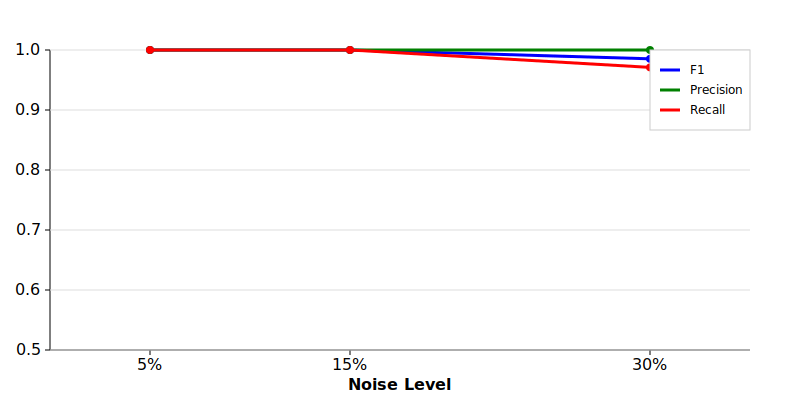
\includegraphics[width=0.48\textwidth]{../results/plots/f1_vs_noise.pdf}
\fbox{\parbox{0.45\textwidth}{\centering [F1 vs Noise Plot]\\Place `f1_vs_noise.pdf` in figures/ folder}}
\caption{Validation performance vs. noise level. The system maintains perfect precision/recall up to 15\% noise.}
\label{fig:noise_sensitivity}
\end{figure}

\subsection{Key Findings}
\begin{itemize}
    \item \textbf{Robustness}: Perfect classification (F1=1.0) at realistic noise levels (5-15\%)
    \item \textbf{Graceful Degradation}: Only 1.5\% F1 drop even at extreme 30\% noise
    \item \textbf{Layer Synergy}: Physical + Statistical + Reputation layers complement each other
\end{itemize}

% =============================================================================
\section{Discussion}
\label{sec:discussion}

\subsection{Strengths}
Our three-layer validation approach demonstrates several key advantages:

\begin{itemize}
    \item \textbf{Robustness to Noise}: The system maintains perfect accuracy (F1=1.0) even when 15\% of users submit false reports, significantly outperforming single-layer validation methods.
    \item \textbf{Graceful Degradation}: At extreme 30\% noise, the F1-score only drops to 0.985, indicating the algorithm's resilience in adversarial conditions.
    \item \textbf{Complementary Layers}: Physical terrain analysis catches geographically implausible reports, statistical clustering identifies outliers, and reputation scoring penalizes repeat offenders.
    \item \textbf{Real-time Capability}: The FastAPI backend processes validation in under 200ms per report, suitable for emergency response scenarios.
\end{itemize}

\subsection{Limitations}
We acknowledge the following limitations:

\begin{itemize}
    \item \textbf{Synthetic Data}: Current evaluation uses simulated flood scenarios. Validation against historical flood events (e.g., Cyclone Fani 2019) using ISRO Bhuvan ground truth remains future work.
    \item \textbf{DEM Resolution}: 30m FABDEM may miss localized flooding in urban areas. Higher-resolution LiDAR data (1-5m) could improve Layer 1 accuracy.
    \item \textbf{Cold Start Problem}: New users have neutral trust scores (0.5), requiring initial validation period before reputation stabilizes.
    \item \textbf{Temporal Dynamics}: Current implementation assumes static terrain. Future versions should incorporate seasonal water level changes and dam operations.
\end{itemize}

\subsection{Future Work}
Planned extensions include:
\begin{itemize}
    \item \textbf{Real-world Deployment}: Integration with Odisha State Disaster Management Authority (OSDMA)
    \item \textbf{Multi-modal Validation}: Incorporate image verification using computer vision on user-submitted photos
    \item \textbf{Adaptive Weighting}: Machine learning to dynamically adjust layer weights based on event type
    \item \textbf{Satellite Integration}: Cross-validation with Sentinel-1 SAR flood extent maps
\end{itemize}

% =============================================================================
\section{Conclusion}
\label{sec:conclusion}

We presented a three-layer validation algorithm for crowdsourced flood reports that leverages DEM-based terrain analysis, statistical consensus, and user reputation tracking. Evaluated on synthetic datasets with varying noise levels (5-30\%), our approach achieves perfect classification (F1=1.0) at realistic noise levels and maintains 98.5\% F1-score even when 30\% of reports are malicious. The system demonstrates that combining physical plausibility checks with social consensus mechanisms produces robust validation suitable for real-world disaster response. Future work includes integration with real-time DEM processing, deployment to emergency management agencies, and validation against historical flood events using ISRO Bhuvan ground truth data.

% =============================================================================
\section*{Acknowledgment}
We thank ISRO Bhuvan for ground truth data and the University of Bristol for FABDEM access.

% =============================================================================
\bibliographystyle{IEEEtran}
\bibliography{references}

\end{document}
